\section{Introduction}

% show diagrams with terms, then show squaring
\frame{
    \frametitle{3D Coupling Dependence}
    \begin{figure}
    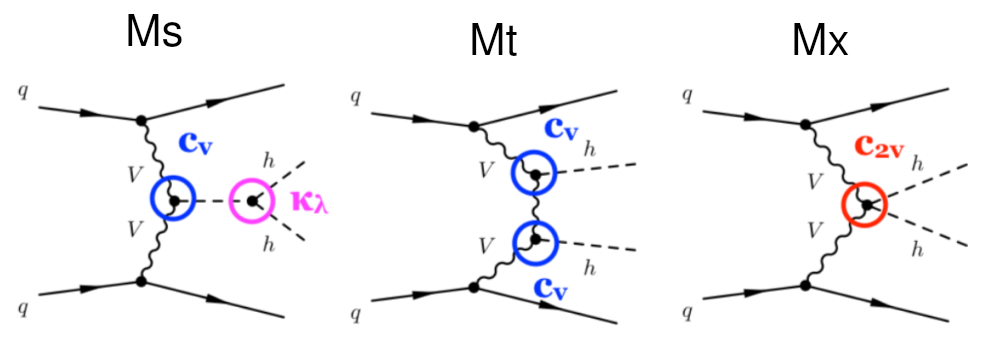
\includegraphics[width=0.6\linewidth,height=0.6\textheight,keepaspectratio]{vbf-hh_diagrams2b}
    \end{figure}
    $ \sigma = | \kv \kl M_s + \kv^2 M_t + \kvv M_x |^2 = $

    \vspace{10mm}

    $ \kv^2 \kl^2 M_s^2 + \kv^4 M_t^2 + \kvv^2 M_x^2 
    + \kv^3 \kl (M_s^* M_t + M_t^* M_s) 
    + \kv \kl \kvv (M_s^* M_x + M_x^* M_s ) 
    + \kv^2 \kvv (M_t^* M_x + M_x^* M_t )$

    \vspace{10mm}

    $ \sigma = \kv^2 \kl^2 a_1 + \kv^4 a_2 + \kvv^2 a_3 + \kv^3 \kl a_4 + \kv \kl \kvv a_5 + \kv^2 \kvv a_6 $
}

\displayonelarge{Negative Weights}{
    Negative weights can appear in the $m_{HH}$ combination. These are unphysical and should be avoided.
}{reco_mHH_cvv1p0cl2p0cv1p0}

\displayonelarge{Extreme Negative Weights}{
    In further regions of the $\kappa$ parameter space, these negative weights can be become dangerously common.
}{preview_reco_mHH_cvv0p0cl-9p0cv1p0_old}

\displayonelarge{Assessing Basis Performance via Negative Weight Integral}{
    Take the surface integral of the number of negative bins at each point at in the $\kappa$ parameter space (mutliplying by the $\kvv \times \kl$ ``area") as a general metric of performance.
}{negative_weights_rank027}
